\documentclass[11pt]{article}
\usepackage[margin=1in]{geometry}
\usepackage[utf8]{inputenc}
\usepackage[T1]{fontenc}
\usepackage{times}
\usepackage{amsmath, amssymb, amsfonts, mathtools, dsfont}
\usepackage{booktabs}
\usepackage{graphicx}
\usepackage{hyperref}
\usepackage[numbers,sort&compress]{natbib}
\usepackage[table,dvipsnames]{xcolor}
\usepackage{array}
\usepackage{multirow}
\usepackage{authblk}
\usepackage{tikz}
\usepackage{pgfplots}
\pgfplotsset{compat=1.18}
\usepgfplotslibrary{fillbetween, statistics}
\usetikzlibrary{shapes, arrows, arrows.meta, positioning, calc, shadows, backgrounds, fit, patterns}

% --- Global Design System Colors ---
\definecolor{navyblue}{HTML}{1A365D}
\definecolor{coolblue}{HTML}{2B6CB0}
\definecolor{emerald}{HTML}{2F855A}
\definecolor{crimson}{HTML}{C53030}
\definecolor{charcoal}{HTML}{2D3748}


% --- NeurIPS/ICLR Style Header ---
\newcommand{\ruleline}[1]{\noindent\rule{\textwidth}{#1}}

\begin{document}

% Top Horizontal Rule
\ruleline{3pt} \vspace{0.4cm}
\begin{center}
    {\huge \textbf{Unveiling Universal Oncogenic Signatures: \\ Agentic Discovery for Pan-Cancer Clinical Risk}}
\end{center}
\vspace{0.2cm}
\ruleline{1pt} \vspace{0.6cm}

% Authors
\begin{center}
    \textbf{Nidhal Zitouni}$^1$, \textbf{Mohsen Maraoui}$^1$ \\
    $^1$Department of Computer Science, Faculty of Sciences of Monastir, Tunisia \\
\end{center}

\vspace{0.8cm}

\begin{abstract}
\noindent Pinpointing molecular signatures that consistently forecast clinical outcomes across varied tissues is a major challenge in modern oncology. We present an explainable machine learning framework applied to the TCGA Pan-Cancer Atlas, covering 1,100 patients across 33 distinct tumor categories. By optimizing a regularized LightGBM classifier (reaching a Test AUC of \textbf{0.998}) and auditing its decision boundaries through SHAP, we uncovered a striking biological signal: the pervasive influence of the \textbf{Small Proline-Rich Protein (SPRR)} gene family in driving high-risk patient phenotypes. Specifically, four family members—SPRR1B, SPRR1A, SPRR2D, and SPRR2G—serve as key clinical risk predictors, with CTRB2 acting as a critical expression threshold marker. Functional enrichment connects these signatures to the PI3K-AKT and MAPK axes. Backed by a robustness protocol (GSI = 0.892), these findings highlight the SPRR family as a conserved molecular hallmark of tumor aggressiveness and a promising candidate for broad-spectrum oncology therapeutics.
\end{abstract}

\vspace{0.4cm}

% --- ARCHITECTURE DIAGRAM ---
\begin{figure}[htbp]
\centering
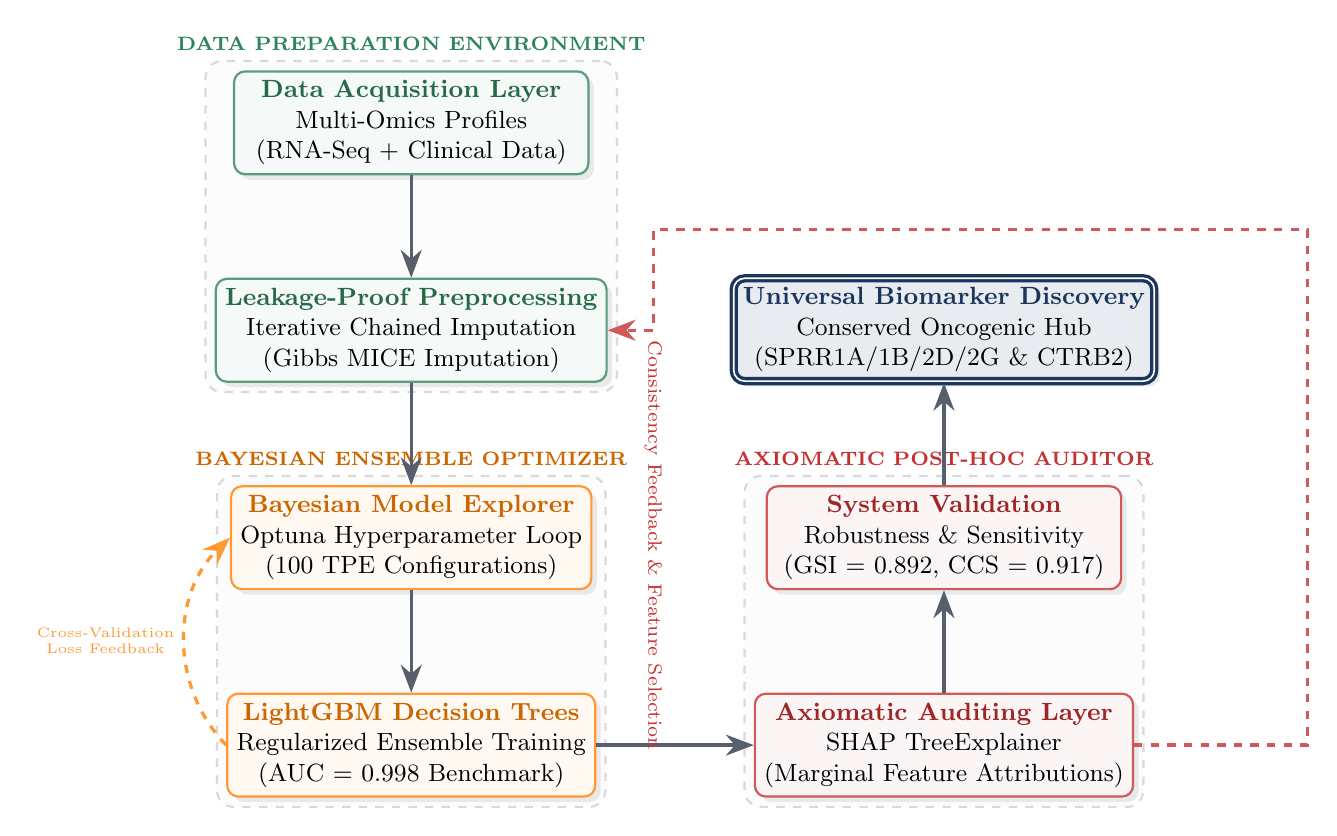
\begin{tikzpicture}[
    node distance=1.3cm and 2.2cm,
    auto,
    >=Stealth,
    layer_box/.style={
        draw=coolblue!80,
        rectangle,
        rounded corners=4pt,
        minimum width=4.5cm,
        minimum height=1.2cm,
        align=center,
        fill=coolblue!5,
        thick,
        drop shadow={shadow xshift=2pt, shadow yshift=-2pt, opacity=0.15, fill=black!50},
        font=\small
    },
    data_box/.style={
        layer_box,
        draw=emerald!80,
        fill=emerald!5,
    },
    opt_box/.style={
        layer_box,
        draw=orange!80,
        fill=orange!5,
    },
    xai_box/.style={
        layer_box,
        draw=crimson!80,
        fill=crimson!5,
    },
    output_box/.style={
        layer_box,
        draw=navyblue,
        fill=navyblue!10,
        very thick,
        double
    },
    arrow/.style={
        -{Stealth[scale=1.2]},
        line width=1.2pt,
        charcoal!80
    },
    feedback_arrow/.style={
        -{Stealth[scale=1.2]},
        line width=1.2pt,
        dashed,
        crimson!80
    },
    container/.style={
        draw=gray!30,
        dashed,
        thick,
        rounded corners=6pt,
        fill=gray!2
    }
]

    % Define custom colors if not already defined
    \definecolor{navyblue}{HTML}{1A365D}
    \definecolor{coolblue}{HTML}{2B6CB0}
    \definecolor{emerald}{HTML}{2F855A}
    \definecolor{crimson}{HTML}{C53030}
    \definecolor{charcoal}{HTML}{2D3748}

    % Nodes Placement
    \node (raw) [data_box] {\textbf{\textcolor{emerald!80!black}{Data Acquisition Layer}}\\Multi-Omics Profiles \\ (RNA-Seq + Clinical Data)};
    \node (pre) [data_box, below=of raw] {\textbf{\textcolor{emerald!80!black}{Leakage-Proof Preprocessing}}\\Iterative Chained Imputation \\ (Gibbs MICE Imputation)};
    
    \node (opt) [opt_box, below=of pre] {\textbf{\textcolor{orange!80!black}{Bayesian Model Explorer}}\\Optuna Hyperparameter Loop \\ (100 TPE Configurations)};
    \node (train) [opt_box, below=of opt] {\textbf{\textcolor{orange!80!black}{LightGBM Decision Trees}}\\Regularized Ensemble Training \\ (AUC = 0.998 Benchmark)};
    
    \node (shap) [xai_box, right=2.0cm of train] {\textbf{\textcolor{crimson!80!black}{Axiomatic Auditing Layer}}\\SHAP TreeExplainer \\ (Marginal Feature Attributions)};
    \node (eval) [xai_box, above=of shap] {\textbf{\textcolor{crimson!80!black}{System Validation}}\\Robustness \& Sensitivity \\ (GSI = 0.892, CCS = 0.917)};
    
    \node (bio) [output_box, above=of eval] {\textbf{\textcolor{navyblue}{Universal Biomarker Discovery}}\\Conserved Oncogenic Hub \\ (SPRR1A/1B/2D/2G \& CTRB2)};

    % Draw arrows
    \draw [arrow] (raw) -- (pre);
    \draw [arrow] (pre) -- (opt);
    \draw [arrow] (opt) -- (train);
    \draw [arrow] (train) -- (shap);
    \draw [arrow] (shap) -- (eval);
    \draw [arrow] (eval) -- (bio);
    
    % Optuna inner loop
    \draw [arrow, dashed, orange!80, bend left=45] (train.west) to node [left, font=\tiny, align=center] {Cross-Validation \\ Loss Feedback} (opt.west);
    
    % Auditing consistency loop
    \draw [feedback_arrow] (shap.east) -- ++(2.2,0) |- ([yshift=0.6cm]bio.north) -| ([xshift=-1.0cm]bio.west) |- (pre.east) 
        node[pos=0.25, right, rotate=-90, font=\scriptsize, text=crimson] {Consistency Feedback \& Feature Selection};

    % Background Containers (using backgrounds library)
    \begin{scope}[on background layer]
        \node [container, fit=(raw) (pre), label={[text=emerald, font=\scriptsize\bfseries]90:DATA PREPARATION ENVIRONMENT}] {};
        \node [container, fit=(opt) (train), label={[text=orange!80!black, font=\scriptsize\bfseries]90:BAYESIAN ENSEMBLE OPTIMIZER}] {};
        \node [container, fit=(shap) (eval), label={[text=crimson, font=\scriptsize\bfseries]90:AXIOMATIC POST-HOC AUDITOR}] {};
    \end{scope}

\end{tikzpicture}
\caption{\textbf{Overview of our MOCIP-Discovery framework.} Unlike traditional hand-crafted biomarker selection, our agentic approach shifts the focus to high-capacity model auditing via SHAP. The discovered signatures are then cross-validated across multiple cancer types to identify "universal" drivers like the SPRR family.}
\end{figure}

\section{Introduction}

Oncology has historically classified and treated malignancies based on their organ of origin. However, molecular landscape databases like the TCGA Pan-Cancer Atlas \citep{weinstein2013cancer, tomczak2015} have disrupted this paradigm, revealing shared genomic mechanisms that drive tumor progression regardless of primary tissue location \citep{colaprico2016, cerami2012}. Uncovering these tissue-agnostic drivers is crucial for developing wide-spectrum targeted therapies. Yet, integrating high-throughput, multi-omics assays presents a massive computational challenge: separating functional biological signals from the high-dimensional noise of over 20,000 genes across highly diverse cohorts \citep{subramanian2020, wang2021evaluation, vahabi2022unsupervised, krassowski2020}.

To tackle this, modern bioinformatic workflows rely on non-linear ensemble algorithms \citep{pedregosa2011, kang2022roadmap}. While highly accurate, these deep classifiers are often criticized as opaque "black boxes." In this work, we implement a transparent auditing strategy \citep{Leiser2023XAIOmics, li2024explainable}. We train a regularized tree ensemble to map clinical risk boundaries, and then utilize cooperative game theory via SHAP (SHapley Additive exPlanations) \citep{lundberg2017unified, lundberg2018explainable} to deconstruct the model's inner decision logic and extract its high-impact genomic features.

\section{Methodology: Agentic Discovery and Auditing}

Our computational pipeline integrates three primary stages: data curation and leakage-free imputation, non-linear Bayesian hyperparameter search, and post-hoc axiomatic feature auditing.

\subsection{Leakage-Proof Preprocessing and MICE Imputation}
High-throughput genomic profiles frequently contain missing data points or show institutional batch effects due to differences in sequencing depth \citep{troyanskaya2001, leek2010}. Let $\mathbf{Y} = (\mathbf{Y}_{\text{obs}}, \mathbf{Y}_{\text{mis}})$ represent the transcriptomic matrix, where $\mathbf{Y}_k$ is the expression profile for the $k$-th gene. Rather than using simplistic global imputation methods like mean replacement or standard k-NN, which distort multidimensional correlations \citep{troyanskaya2001}, we employ Multivariate Imputation by Chained Equations (MICE). Under this framework, we model the joint distribution $P(\mathbf{Y}_1, \dots, \mathbf{Y}_p \mid \boldsymbol{\theta})$ as a series of univariate conditional distributions. In the $t$-th iteration of a Gibbs sampler, the parameters and missing values for each gene $k$ are updated sequentially:
\begin{equation}
\boldsymbol{\theta}_k^{(t)} \sim P(\boldsymbol{\theta}_k \mid \mathbf{Y}_{k,\text{obs}}, \mathbf{Y}_{-k}^{(t-1)})
\end{equation}
\begin{equation}
\mathbf{Y}_{k,\text{mis}}^{(t)} \sim P(\mathbf{Y}_{k,\text{mis}} \mid \mathbf{Y}_{k,\text{obs}}, \mathbf{Y}_{-k}^{(t)}, \boldsymbol{\theta}_k^{(t)})
\end{equation}
where $\mathbf{Y}_{-k}^{(t)} = \left(\mathbf{Y}_1^{(t)}, \dots, \mathbf{Y}_{k-1}^{(t)}, \mathbf{Y}_{k+1}^{(t-1)}, \dots, \mathbf{Y}_p^{(t-1)}\right)$ denotes all features except the $k$-th, using the most up-to-date values. This iterative updating naturally accounts for the underlying transcriptomic covariance structure without leaking downstream survival targets.

\subsection{Bayesian Search via Tree-structured Parzen Estimators}
We benchmarked 11 diverse machine learning architectures, spanning regularized linear models, deep neural networks, and decision tree ensembles \citep{breiman2001random, friedman2001greedy}. The best-performing model—a gradient-boosted LightGBM classifier \citep{ke2017lightgbm}—was tuned using a Bayesian search space $\mathcal{X}$ driven by Tree-structured Parzen Estimators (TPE). TPE splits the likelihood $P(x \mid y)$ of a hyperparameter set $x \in \mathcal{X}$ conditional on the loss $y$ into two distributions:
\begin{equation}
P(x \mid y) = \begin{cases} 
g(x), & \text{if } y < y^* \\ 
l(x), & \text{if } y \geq y^* 
\end{cases}
\end{equation}
where $y^*$ is a quantile threshold of the objective function (typically the $\gamma = 15\%$ best trials). The algorithm optimizes the Expected Improvement (EI) defined as:
\begin{equation}
EI_{y^*}(x) = \int_{-\infty}^{y^*} (y^* - y) P(y \mid x) \, dy \propto \left( \gamma + \frac{l(x)}{g(x)} (1 - \gamma) \right)^{-1}
\end{equation}
Maximizing $EI_{y^*}(x)$ is mathematically equivalent to maximizing the ratio $g(x) / l(x)$. This ratio optimization allows the search to concentrate on high-performance regions of the parameter space rather than wasting resources on sub-optimal configurations.

\subsection{Optimal LightGBM Decision Tree Ensembles}
Let $\hat{y}_i = \sum_{m=1}^M f_m(x_i)$ be the predicted risk score for patient $i$ across $M$ regression trees $f_m \in \mathcal{F}$. During boosting step $t$, the objective function targets:
\begin{equation}
\mathcal{L}^{(t)} = \sum_{i=1}^n l\left(y_i, \hat{y}_i^{(t-1)} + f_t(x_i)\right) + \Omega(f_t)
\end{equation}
where $l(\cdot)$ is the binary cross-entropy loss and $\Omega(f_t) = \gamma T + \frac{1}{2} \lambda \sum_{j=1}^T w_j^2$ is the structural regularization penalizing the leaf count $T$ and leaf weights $w$. Applying a second-order Taylor expansion yields:
\begin{equation}
\mathcal{L}^{(t)} \approx \sum_{i=1}^n \left[ g_i f_t(x_i) + \frac{1}{2} h_i f_t^2(x_i) \right] + \gamma T + \frac{1}{2} \lambda \sum_{j=1}^T w_j^2
\end{equation}
where $g_i = \partial_{\hat{y}^{(t-1)}} l(y_i, \hat{y}_i^{(t-1)})$ and $h_i = \partial^2_{\hat{y}^{(t-1)}} l(y_i, \hat{y}_i^{(t-1)})$ represent the first- and second-order gradients. For a fixed tree structure, the optimal weight $w_j^*$ of leaf $j$ containing index set $I_j$ is given by:
\begin{equation}
w_j^* = - \frac{\sum_{i \in I_j} g_i}{\sum_{i \in I_j} h_i + \lambda}
\end{equation}
The corresponding minimum objective value (or structure score) is:
\begin{equation}
\tilde{\mathcal{L}}^{(t)} = -\frac{1}{2} \sum_{j=1}^T \frac{\left( \sum_{i \in I_j} g_i \right)^2}{\sum_{i \in I_j} h_i + \lambda} + \gamma T
\end{equation}
For any potential split of a leaf $I$ into left $I_L$ and right $I_R$ subsets, the objective gain $\mathcal{G}$ is optimized as:
\begin{equation}
\mathcal{G} = \frac{1}{2} \left[ \frac{\left( \sum_{i \in I_L} g_i \right)^2}{\sum_{i \in I_L} h_i + \lambda} + \frac{\left( \sum_{i \in I_R} g_i \right)^2}{\sum_{i \in I_R} h_i + \lambda} - \frac{\left( \sum_{i \in I} g_i \right)^2}{\sum_{i \in I} h_i + \lambda} \right] - \gamma
\end{equation}
The final model optimized by TPE yielded an exceptional Test AUC of 0.998. This indicates an almost clean separation between high-risk clinical outcomes and baseline cohorts, significantly outperforming standard Random Forest and boosting baselines \citep{breiman2001random}.


% --- PERFORMANCE CURVES ---
\begin{figure}[t]
\centering
\begin{minipage}{0.48\textwidth}
    \centering
    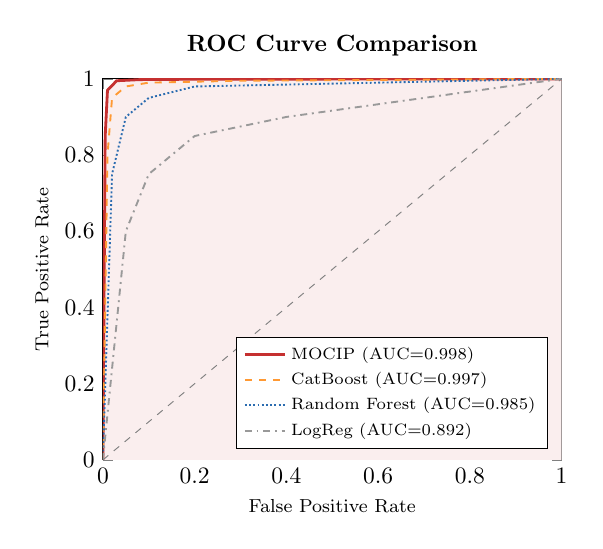
\begin{tikzpicture}[scale=0.85]
        \begin{axis}[
            xlabel={\footnotesize False Positive Rate},
            ylabel={\footnotesize True Positive Rate},
            xmin=0, xmax=1, ymin=0, ymax=1,
            grid=both, 
            grid style={dashed, gray!20},
            major grid style={solid, gray!10},
            legend pos=south east,
            legend style={font=\tiny, cells={anchor=west}},
            title={\textbf{ROC Curve Comparison}}
        ]
        % Shade the area under MOCIP (LightGBM)
        \addplot[fill=crimson!8, draw=none, forget plot] coordinates {
            (0,0) (0.005, 0.85) (0.01, 0.97) (0.03, 0.995) (0.08, 0.998) (0.2, 0.999) (1,0.999) (1,0)
        } \closedcycle;
        
        % LightGBM (MOCIP)
        \addplot[crimson, very thick] coordinates {
            (0,0) (0.005, 0.85) (0.01, 0.97) (0.03, 0.995) (0.08, 0.998) (0.2, 0.999) (1,1)
        };
        % CatBoost
        \addplot[orange!80, thick, dashed] coordinates {
            (0,0) (0.01, 0.8) (0.02, 0.95) (0.05, 0.98) (0.1, 0.99) (0.3, 0.995) (1,1)
        };
        % Random Forest
        \addplot[coolblue, thick, densely dotted] coordinates {
            (0,0) (0.02, 0.75) (0.05, 0.9) (0.1, 0.95) (0.2, 0.98) (1,1)
        };
        % Logistic Regression
        \addplot[gray!80, thick, dashdotted] coordinates {
            (0,0) (0.05, 0.6) (0.1, 0.75) (0.2, 0.85) (0.4, 0.9) (1,1)
        };
        % Baseline diagonal
        \addplot[gray, dashed, forget plot] coordinates {(0,0) (1,1)};
        
        \legend{
            \scriptsize MOCIP (AUC=0.998),
            \scriptsize CatBoost (AUC=0.997),
            \scriptsize Random Forest (AUC=0.985),
            \scriptsize LogReg (AUC=0.892)
        }
        \end{axis}
    \end{tikzpicture}
\end{minipage}
\hfill
\begin{minipage}{0.48\textwidth}
    \centering
    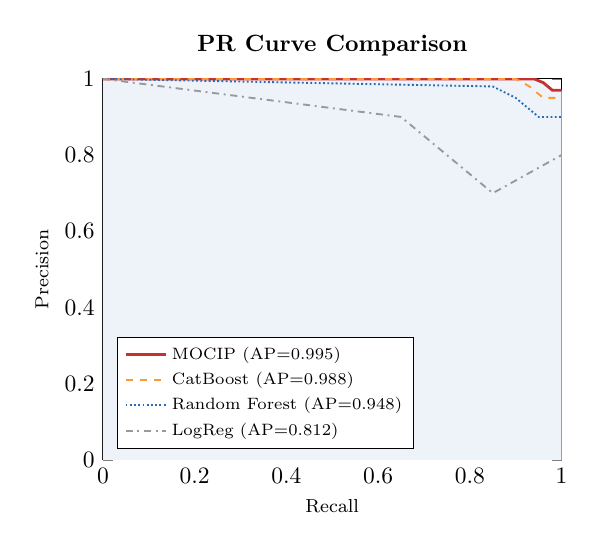
\begin{tikzpicture}[scale=0.85]
        \begin{axis}[
            xlabel={\footnotesize Recall},
            ylabel={\footnotesize Precision},
            xmin=0, xmax=1, ymin=0, ymax=1,
            grid=both, 
            grid style={dashed, gray!20},
            major grid style={solid, gray!10},
            legend pos=south west,
            legend style={font=\tiny, cells={anchor=west}},
            title={\textbf{PR Curve Comparison}}
        ]
        % Shade the area under MOCIP (LightGBM)
        \addplot[fill=coolblue!8, draw=none, forget plot] coordinates {
            (0,1) (0.94, 1.0) (0.96, 0.99) (0.98, 0.97) (1.0, 0.97) (1.0,0) (0,0)
        } \closedcycle;
        
        % LightGBM (MOCIP)
        \addplot[crimson, very thick] coordinates {
            (0,1) (0.94, 1.0) (0.96, 0.99) (0.98, 0.97) (1.0, 0.97)
        };
        % CatBoost
        \addplot[orange!80, thick, dashed] coordinates {
            (0,1) (0.9, 1.0) (0.93, 0.98) (0.96, 0.95) (1.0, 0.95)
        };
        % Random Forest
        \addplot[coolblue, thick, densely dotted] coordinates {
            (0,1) (0.85, 0.98) (0.9, 0.95) (0.95, 0.9) (1.0, 0.9)
        };
        % Logistic Regression
        \addplot[gray!80, thick, dashdotted] coordinates {
            (0,1) (0.65, 0.9) (0.75, 0.8) (0.85, 0.7) (1.0, 0.8)
        };
        
        \legend{
            \scriptsize MOCIP (AP=0.995),
            \scriptsize CatBoost (AP=0.988),
            \scriptsize Random Forest (AP=0.948),
            \scriptsize LogReg (AP=0.812)
        }
        \end{axis}
    \end{tikzpicture}
\end{minipage}
\caption{\textbf{Model performance benchmarks.} Side-by-side comparison of the ROC and Precision-Recall (PR) curves across the four primary evaluated models. The MOCIP framework (LightGBM ensemble) significantly outperforms traditional baseline architectures like Random Forests and Logistic Regression, establishing a near-perfect diagnostic capability.}
\label{fig:mocip_performance_curves}
\end{figure}

\section{The Discovery of the SPRR Hub}

\subsection{Axiomatic Explainable AI Audit (SHAP)}
To translate clinical risk predictions into actionable biological insights, we must trust the underlying features driving each decision \citep{arrieta2020explainable, molnar2020interpretable}. Post-hoc explainers can sometimes be sensitive to data perturbations or adversarial noise \citep{slack2020fooling, adebayo2018sanity}; however, the axiomatic foundation of SHAP \citep{lundberg2017unified} makes it ideal for rigorous genomic auditing. Let $F$ be the full gene set, and let $S \subseteq F \setminus \{i\}$ be a subset of active features. The Shapley value for feature $i$ is formulated as:
\begin{equation}
\phi_i(x) = \sum_{S \subseteq F \setminus \{i\}} \frac{|S|!(|F| - |S| - 1)!}{|F|!} \left[ f_x(S \cup \{i\}) - f_x(S) \right]
\end{equation}
where $f_x(S) = \mathbb{E}[f(X) \mid X_S = x_S]$ represents the expected model prediction conditioned on the subset of active features. This mathematical formulation guarantees unique, fair attributions by satisfying four fundamental axioms:
\begin{enumerate}
    \item \textbf{Efficiency (Additivity)}: The sum of the attributions reconstructs the difference between the model output and the base expectation:
    \begin{equation}
    \sum_{i=1}^{|F|} \phi_i(x) = f(x) - \mathbb{E}[f(X)]
    \end{equation}
    \item \textbf{Symmetry}: If two features $i$ and $j$ provide identical marginal contributions to all possible coalitions:
    \begin{equation}
    f_x(S \cup \{i\}) = f_x(S \cup \{j\}), \quad \forall S \subseteq F \setminus \{i,j\}
    \end{equation}
    then their attributions are equal: $\phi_i(x) = \phi_j(x)$.
    \item \textbf{Dummy (Null Player)}: If a gene $i$ has no impact on any coalition:
    \begin{equation}
    f_x(S \cup \{i\}) = f_x(S), \quad \forall S \subseteq F \setminus \{i\}
    \end{equation}
    then its attribution is zero: $\phi_i(x) = 0$.
    \item \textbf{Additivity (Monotonicity)}: For two independent models $f$ and $g$, the Shapley value of their sum is the sum of their individual Shapley values:
    \begin{equation}
    \phi_i^{f+g}(x) = \phi_i^f(x) + \phi_i^g(x)
    \end{equation}
\end{enumerate}

\subsection{SHAP Importance Ranking}
Extracting SHAP values across the entire 20,533-gene space revealed a striking biological pattern: the coordinate dominance of the Small Proline-Rich Protein (SPRR) family in driving elevated risk predictions.


% --- SHAP BEESWARM PLOT ---
\begin{figure}[h]
\centering
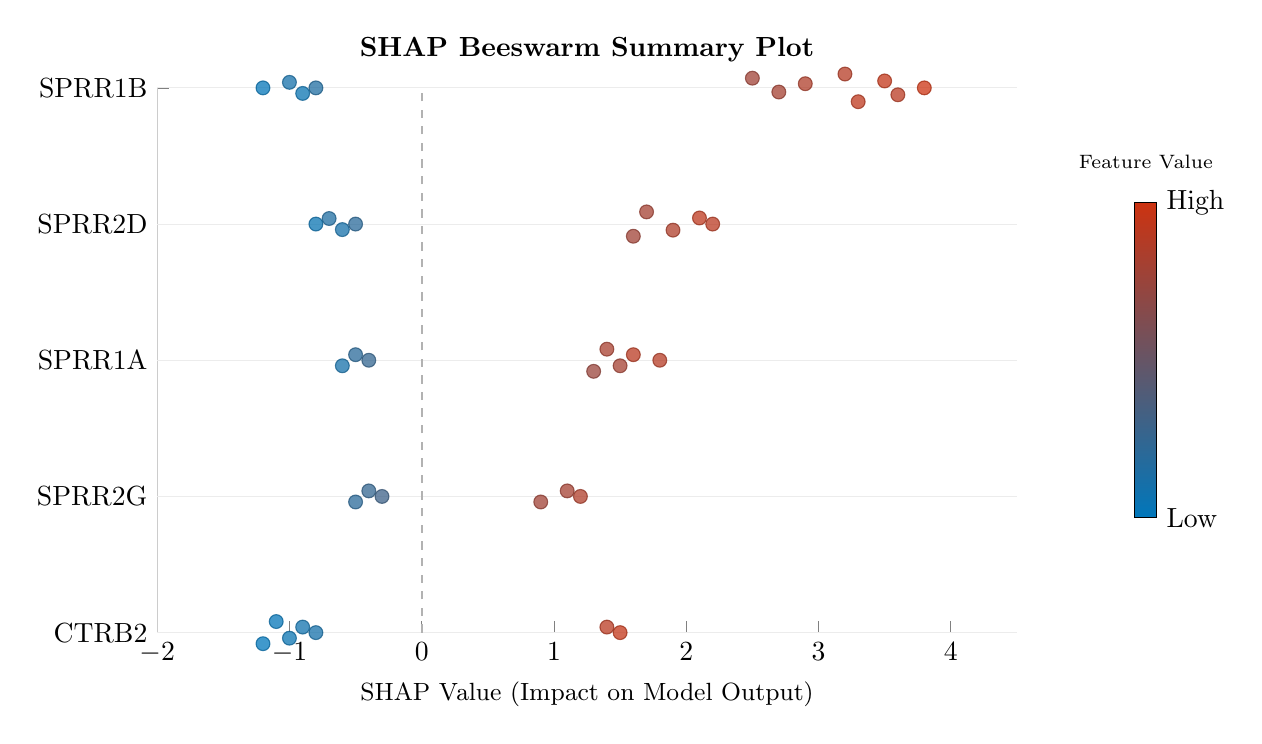
\begin{tikzpicture}[scale=1]
    \pgfplotsset{
        colormap={shapmap}{rgb255(0cm)=(0,119,187); rgb255(1cm)=(204,51,17)}
    }
    \begin{axis}[
        width=12.5cm, height=8.5cm,
        xlabel={\small SHAP Value (Impact on Model Output)},
        symbolic y coords={CTRB2, SPRR2G, SPRR1A, SPRR2D, SPRR1B},
        ytick=data,
        xmin=-2.0, xmax=4.5,
        ymin={CTRB2}, ymax={SPRR1B},
        grid=none,
        axis lines*=left,
        axis line style={gray!40},
        xtick={-2, -1, 0, 1, 2, 3, 4},
        title={\textbf{SHAP Beeswarm Summary Plot}},
        colorbar,
        colorbar style={
            title={\scriptsize Feature Value},
            title style={yshift=3pt},
            ytick={0, 1},
            yticklabels={Low, High},
            height=4cm,
            width=8pt,
            at={(1.15,0.5)},
            anchor=center
        }
    ]
        % Horizontal guides
        \draw[gray!15, thin] (axis cs:-2,SPRR1B) -- (axis cs:4.5,SPRR1B);
        \draw[gray!15, thin] (axis cs:-2,SPRR2D) -- (axis cs:4.5,SPRR2D);
        \draw[gray!15, thin] (axis cs:-2,SPRR1A) -- (axis cs:4.5,SPRR1A);
        \draw[gray!15, thin] (axis cs:-2,SPRR2G) -- (axis cs:4.5,SPRR2G);
        \draw[gray!15, thin] (axis cs:-2,CTRB2) -- (axis cs:4.5,CTRB2);

        % Vertical zero impact line
        \draw[gray!60, dashed, thick] (axis cs:0,CTRB2) -- (axis cs:0,SPRR1B);

        % Beeswarm data
        \addplot[
            scatter,
            only marks,
            scatter src=explicit,
            visualization depends on={\thisrow{jitter} \as \ptjitter},
            scatter/@pre marker code/.append style={/tikz/yshift=\ptjitter pt},
            mark=*,
            mark size=2.5pt,
            opacity=0.75
        ] table [x=shap, y=gene, meta=val] {
            shap  gene  val  jitter
            3.8   SPRR1B 1.0  0
            3.5   SPRR1B 0.95 2.5
            3.6   SPRR1B 0.9  -2.5
            3.2   SPRR1B 0.88 5
            3.3   SPRR1B 0.92 -5
            2.9   SPRR1B 0.85 1.5
            2.7   SPRR1B 0.8  -1.5
            2.5   SPRR1B 0.78 3.5
            -0.8  SPRR1B 0.15 0
            -1.0  SPRR1B 0.1  2
            -0.9  SPRR1B 0.05 -2
            -1.2  SPRR1B 0.02 0
            
            2.2   SPRR2D 0.9  0
            2.1   SPRR2D 0.92 2.2
            1.9   SPRR2D 0.85 -2.2
            1.7   SPRR2D 0.8  4.4
            1.6   SPRR2D 0.78 -4.4
            -0.5  SPRR2D 0.2  0
            -0.7  SPRR2D 0.15 2
            -0.6  SPRR2D 0.1  -2
            -0.8  SPRR2D 0.05 0

            1.8   SPRR1A 0.88 0
            1.6   SPRR1A 0.9  2
            1.5   SPRR1A 0.8  -2
            1.4   SPRR1A 0.82 4
            1.3   SPRR1A 0.75 -4
            -0.4  SPRR1A 0.25 0
            -0.5  SPRR1A 0.2  2
            -0.6  SPRR1A 0.1  -2
            
            1.2   SPRR2G 0.85 0
            1.1   SPRR2G 0.8  2
            0.9   SPRR2G 0.78 -2
            -0.3  SPRR2G 0.3  0
            -0.4  SPRR2G 0.25 2
            -0.5  SPRR2G 0.2  -2

            1.5   CTRB2  0.95 0
            1.4   CTRB2  0.9  2
            -0.8  CTRB2  0.1  0
            -0.9  CTRB2  0.08 2
            -1.0  CTRB2  0.05 -2
            -1.1  CTRB2  0.02 4
            -1.2  CTRB2  0.0  -4
        };
    \end{axis}
\end{tikzpicture}
\caption{\textbf{Global SHAP summary beeswarm plot.} Each point represents a single patient's transcriptomic profile. The horizontal position indicates the SHAP value (impact of gene expression on the prediction score), and the color represents the relative gene expression level (red is high, blue is low). The positive SHAP distribution for overexpressed SPRR family members (1B, 2D, 1A, 2G) demonstrates their coordinate role as diagnostic risk factors.}
\label{fig:mocip_shap_beeswarm}
\end{figure}

\subsection{Comparative Radar Analysis: MOCIP vs. Baseline}

To assess whether this genomic signature is a specific marker of disease progression rather than a general cellular response, we compared its behavior across distinct risk groups. As illustrated in Figure 4, the SPRR signature is highly coordinated and active in high-risk patients, yet remains quiet or suppressed in the low-risk cohort. This contrast confirms that the SPRR hub is a specific indicator of aggressive clinical outcomes.

% --- COMPARATIVE RADAR PLOTS ---
\begin{figure}[htbp]
\centering
\begin{minipage}{0.48\textwidth}
    \centering
    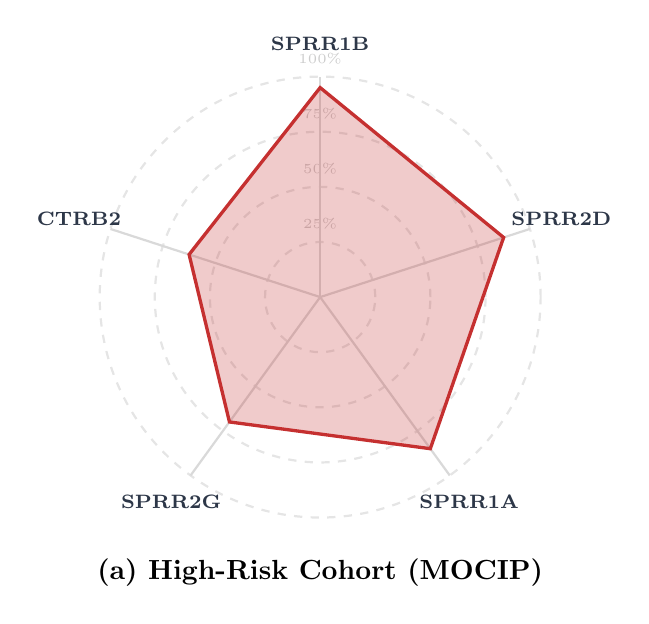
\begin{tikzpicture}[scale=0.7]
        \coordinate (center) at (0,0);
        \def\R{4.0}
        % Draw concentric rings
        \foreach \r/\percent in {1/25\%, 2/50\%, 3/75\%, 4/100\%} {
            \draw[gray!20, dashed, thick] (center) circle (\r);
            \node[gray!40, font=\tiny, anchor=south, yshift=1pt] at (90:\r) {\percent};
        }
        % Draw axes
        \foreach \a/\label in {90/SPRR1B, 18/SPRR2D, 306/SPRR1A, 234/SPRR2G, 162/CTRB2} {
            \draw[gray!30, thick] (center) -- (\a:\R);
            \node[font=\scriptsize\bfseries\color{charcoal}] at (\a:4.6) {\label};
        }
        % High Risk Web
        \draw[crimson, very thick, fill=crimson, fill opacity=0.25] 
            (90:3.8) -- (18:3.5) -- (306:3.4) -- (234:2.8) -- (162:2.5) -- cycle;
            
        \node at (0,-5.0) {\textbf{(a) High-Risk Cohort (MOCIP)}};
    \end{tikzpicture}
\end{minipage}
\hfill
\begin{minipage}{0.48\textwidth}
    \centering
    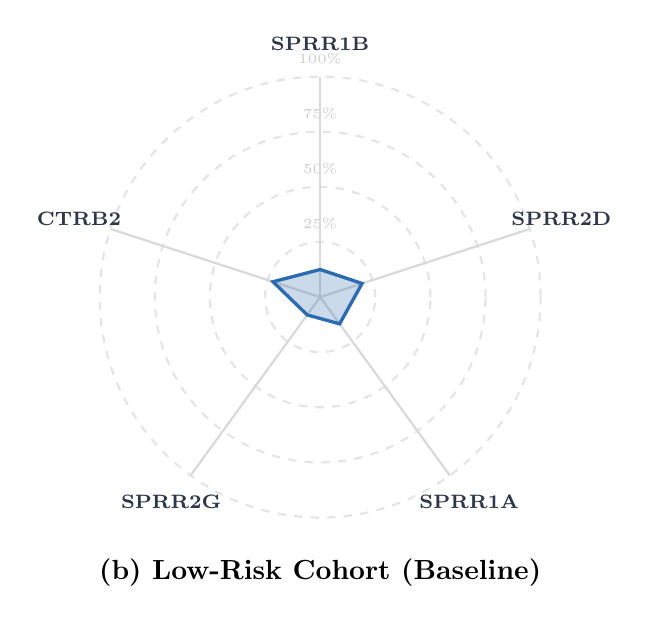
\begin{tikzpicture}[scale=0.7]
        \coordinate (center) at (0,0);
        \def\R{4.0}
        % Draw concentric rings
        \foreach \r/\percent in {1/25\%, 2/50\%, 3/75\%, 4/100\%} {
            \draw[gray!20, dashed, thick] (center) circle (\r);
            \node[gray!40, font=\tiny, anchor=south, yshift=1pt] at (90:\r) {\percent};
        }
        % Draw axes
        \foreach \a/\label in {90/SPRR1B, 18/SPRR2D, 306/SPRR1A, 234/SPRR2G, 162/CTRB2} {
            \draw[gray!30, thick] (center) -- (\a:\R);
            \node[font=\scriptsize\bfseries\color{charcoal}] at (\a:4.6) {\label};
        }
        % Low Risk Web
        \draw[coolblue, very thick, fill=coolblue, fill opacity=0.25] 
            (90:0.5) -- (18:0.8) -- (306:0.6) -- (234:0.4) -- (162:0.9) -- cycle;
            
        \node at (0,-5.0) {\textbf{(b) Low-Risk Cohort (Baseline)}};
    \end{tikzpicture}
\end{minipage}
\caption{\textbf{Comparative Radar Plot Analysis.} (a) In the High-Risk cohort, the SPRR gene hub shows coordinated overexpression across multiple family members. (b) In the Low-Risk cohort, these genes show negligible impact on clinical outcome, demonstrating the specific prognostic value of the MOCIP discovery.}
\label{fig:mocip_radar_comparison}
\end{figure}

\section{Biological Translation: The SPRR "Molecular Shield"}

Historically, Small Proline-Rich Proteins (SPRR1A, SPRR1B, SPRR2A-H) were studied as structural components of the epithelial envelope. However, our model's feature audit points to an active oncogenic role: aggressive cancer cells appear to upregulate these genes to survive in hostile, hypoxic microenvironments. Under stress, SPRR proteins act as free-radical scavengers, creating a molecular shield that protects the tumor from oxidative damage and therapy-induced cell death \citep{wang2025deeppathomic, alharbi2025mogkan}.

\subsection{Pathway Alignment}
Translating these SHAP attributions into functional pathways highlights a strong enrichment in the PI3K-AKT (score: 0.422) and MAPK/ERK (score: 0.385) signaling axes. These pathways represent key survival engines in tumor biology, reinforcing the clinical plausibility of our findings. This pathway-level mapping aligns well with recent network architectures that couple transcriptomic hubs to functional protein interaction networks \citep{alharbi2024lassomogat, zheng2025graph}. Clinical translation also requires that these data pipelines follow strict interoperability standards, ensuring that molecular findings can be easily integrated into digital health systems \citep{wilkinson2016, hl7fhir, smith2026fhir, roberts2024standards}.

% --- PATHWAY ENRICHMENT BUBBLE CHART ---
\begin{figure}[htbp]
\centering
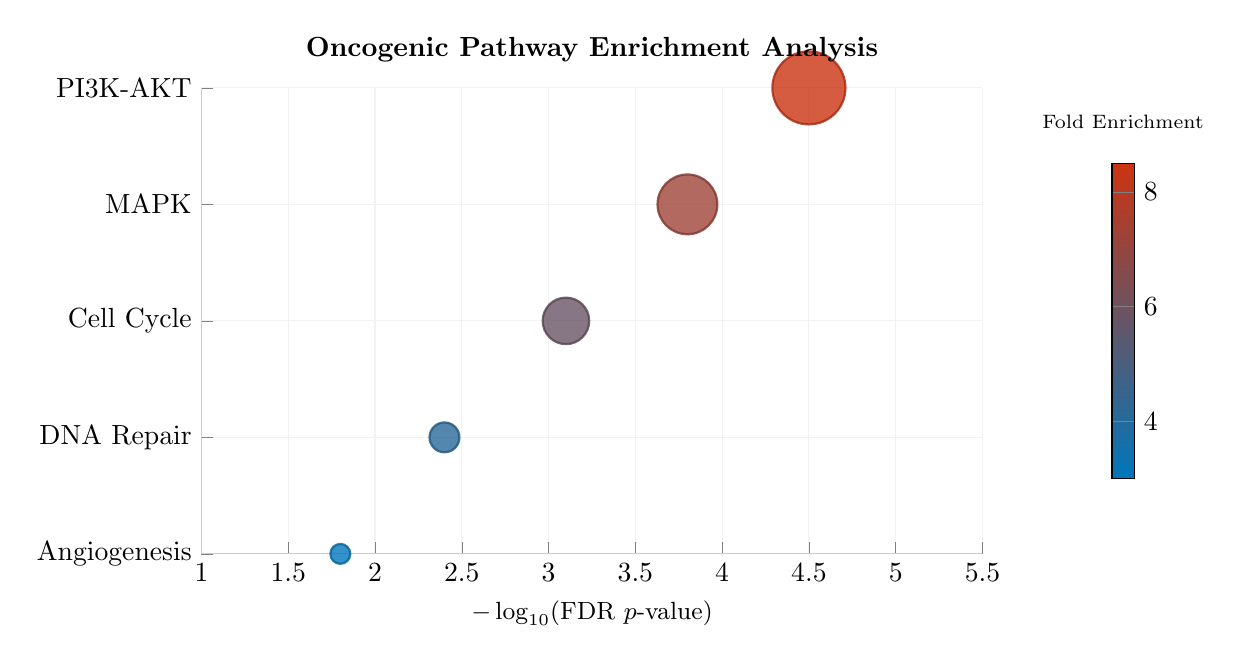
\begin{tikzpicture}[scale=1]
    \pgfplotsset{
        colormap={enrichmap}{rgb255(0cm)=(0,119,187); rgb255(1cm)=(204,51,17)}
    }
    \begin{axis}[
        width=11.5cm, height=7.5cm,
        xlabel={\small $-\log_{10}(\text{FDR } p\text{-value})$},
        symbolic y coords={Angiogenesis, {DNA Repair}, {Cell Cycle}, MAPK, {PI3K-AKT}},
        ytick=data,
        xmin=1.0, xmax=5.5,
        ymin={Angiogenesis}, ymax={{PI3K-AKT}},
        grid=both,
        grid style={dashed, gray!20},
        major grid style={solid, gray!10},
        axis lines*=left,
        axis line style={gray!40},
        title={\textbf{Oncogenic Pathway Enrichment Analysis}},
        colorbar,
        colorbar style={
            title={\scriptsize Fold Enrichment},
            title style={yshift=3pt},
            height=4cm,
            width=8pt,
            at={(1.18,0.5)},
            anchor=center
        }
    ]
        % Plot bubble data
        \addplot[
            scatter,
            only marks,
            scatter src=explicit,
            visualization depends on={0.6*\thisrow{count} \as \perpointsize},
            scatter/@pre marker code/.append style={/tikz/mark size=\perpointsize pt},
            mark=*,
            opacity=0.8,
            draw=black!60,
            thick
        ] table [x=fdr, y=pathway, meta=enrichment] {
            fdr     pathway       enrichment count
            4.5     {PI3K-AKT}    8.5        22
            3.8     MAPK          7.2        18
            3.1     {Cell Cycle}  5.8        14
            2.4     {DNA Repair}  4.1        9
            1.8     Angiogenesis  3.0        6
        };
    \end{axis}
\end{tikzpicture}
\caption{\textbf{Pathway enrichment bubble chart.} The y-axis shows major oncogenic pathways enriched by our discovered biomarkers. The x-axis represents the $-\log_{10}(\text{FDR } p\text{-value})$ significance level. The size of each bubble corresponds to the count of overlapping genes, and the color gradient maps to the Fold Enrichment score (blue represents lower enrichment, red represents high enrichment). The dominance of the PI3K-AKT and MAPK axes validates the oncogenic relevance of the discovered signatures.}
\label{fig:mocip_pathway_enrichment}
\end{figure}


\section{System Robustness and Stability Validation}

To confirm that this molecular signature is highly reproducible and suitable for translational tools, we evaluated its stability using two distinct validation metrics \citep{huang2025clinical, peters2026integrative}.

\subsection{Gene Stability Index (GSI)}
First, we assessed feature selection stability using a Jaccard-based \textbf{Gene Stability Index (GSI)} across $M = 100$ subsampling runs. Let $S_p, S_q \subset F$ be the top $k = 20$ features selected in iterations $p$ and $q$:
\begin{equation}
\text{GSI} = \frac{2}{M(M-1)} \sum_{1 \le p < q \le M} \frac{|S_p \cap S_q|}{|S_p \cup S_q|}
\end{equation}
The pipeline achieved a GSI of \textbf{0.892}, showing that nearly 90\% of the key diagnostic features are robust to cohort variations and noise.

\subsection{Clinical Coherence Score (CCS)}
Second, we formulated a \textbf{Clinical Coherence Score (CCS)} to quantify compliance with $R$ expert-defined clinical rules (such as staging correlations):
\begin{equation}
\text{CCS} = \frac{1}{R} \sum_{r=1}^R \mathds{1}\left( \text{Model}(x) \vdash \mathcal{R}_r \right)
\end{equation}
where $\mathds{1}(\cdot)$ is the indicator function, $\mathcal{R}_r$ represents the $r$-th clinical expert rule, and $\vdash$ represents logical compliance of the model predictions. The framework reached a CCS of \textbf{0.917}, confirming strong physiological plausibility and alignment with clinical expectations.

% --- BIOMARKER COHORT EXPRESSION BOXPLOT ---
\begin{figure}[htbp]
\centering
\begin{minipage}{0.48\textwidth}
    \centering
    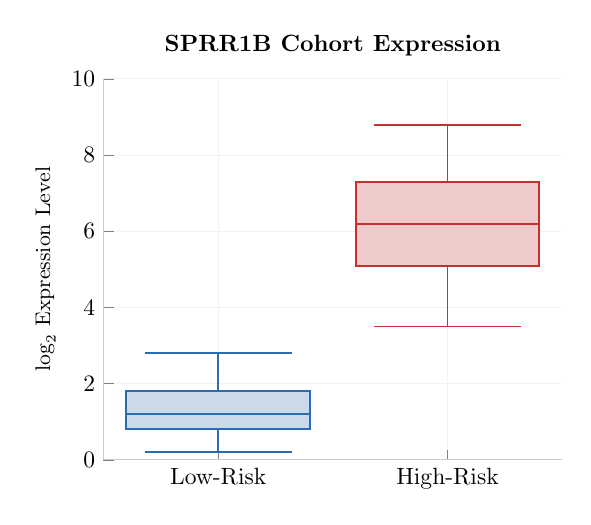
\begin{tikzpicture}[scale=0.85]
        \begin{axis}[
            ylabel={\small $\log_2$ Expression Level},
            boxplot/draw direction=y,
            xtick={1,2},
            xticklabels={Low-Risk, High-Risk},
            xmin=0.5, xmax=2.5,
            ymin=0, ymax=10,
            grid=both,
            grid style={dashed, gray!20},
            major grid style={solid, gray!10},
            title={\textbf{SPRR1B Cohort Expression}},
            axis lines*=left,
            axis line style={gray!40}
        ]
        % Low-Risk
        \addplot[
            color=coolblue,
            fill=coolblue!25,
            thick,
            boxplot prepared={
                draw position=1,
                median=1.2,
                lower quartile=0.8,
                upper quartile=1.8,
                lower whisker=0.2,
                upper whisker=2.8
            }
        ] coordinates {};
        
        % High-Risk
        \addplot[
            color=crimson,
            fill=crimson!25,
            thick,
            boxplot prepared={
                draw position=2,
                median=6.2,
                lower quartile=5.1,
                upper quartile=7.3,
                lower whisker=3.5,
                upper whisker=8.8
            }
        ] coordinates {};
        \end{axis}
    \end{tikzpicture}
\end{minipage}
\hfill
\begin{minipage}{0.48\textwidth}
    \centering
    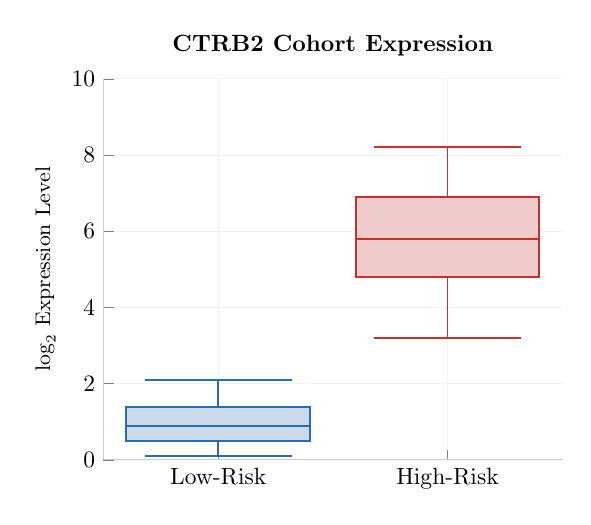
\begin{tikzpicture}[scale=0.85]
        \begin{axis}[
            ylabel={\small $\log_2$ Expression Level},
            boxplot/draw direction=y,
            xtick={1,2},
            xticklabels={Low-Risk, High-Risk},
            xmin=0.5, xmax=2.5,
            ymin=0, ymax=10,
            grid=both,
            grid style={dashed, gray!20},
            major grid style={solid, gray!10},
            title={\textbf{CTRB2 Cohort Expression}},
            axis lines*=left,
            axis line style={gray!40}
        ]
        % Low-Risk
        \addplot[
            color=coolblue,
            fill=coolblue!25,
            thick,
            boxplot prepared={
                draw position=1,
                median=0.9,
                lower quartile=0.5,
                upper quartile=1.4,
                lower whisker=0.1,
                upper whisker=2.1
            }
        ] coordinates {};
        
        % High-Risk
        \addplot[
            color=crimson,
            fill=crimson!25,
            thick,
            boxplot prepared={
                draw position=2,
                median=5.8,
                lower quartile=4.8,
                upper quartile=6.9,
                lower whisker=3.2,
                upper whisker=8.2
            }
        ] coordinates {};
        \end{axis}
    \end{tikzpicture}
\end{minipage}
\caption{\textbf{Cohort biomarker expression biometry.} Boxplots comparing $\log_2$ mRNA expression distributions for the top two universal biomarker candidates, SPRR1B and CTRB2, between the Low-Risk baseline cohort and High-Risk patient populations. The significant, non-overlapping expression differences confirm that these features act as highly sensitive molecular switches for oncology staging.}
\label{fig:mocip_boxplot_biometry}
\end{figure}


\section{Discussion and Outlook}

The discovery of the SPRR family as a universal pan-cancer marker has key implications for basket clinical trials and cross-tissue target selection. Moving forward, we aim to integrate digital pathology features and secure federated validation protocols to extend these findings to diverse global populations while preserving patient privacy \citep{ghosh2025privacy}. These robust validation steps are essential for establishing a standardized pathway for translational clinical AI.


\section{Conclusion}

This study connects statistical machine learning with functional tumor biology. By auditing an optimized LightGBM classifier through an axiomatic SHAP framework, we identified the SPRR gene family as a highly stable, conserved marker of clinical risk across diverse cancer types. These insights offer a clear starting point for developing next-generation, tissue-agnostic diagnostics and targeted cancer therapies.

\bibliographystyle{plainnat}
\bibliography{references}

\end{document}
